\documentclass[10pt,openright,twoside,french]{book}

\usepackage{marvosym}
\input philippe2013
\input philippe2013_activites

\usepackage{docmute}

\pagestyle{empty}

\begin{document}

%_________________________________________
%===    Page de garde
%------------------------------------------------------

\frontmatter

\titlepage{
\begin{center}
{\Large\bfseries\color{\MaCouleur} Philippe \bsc{De Sousa}}

\vspace*{\stretch{1}}

\begin{tikzpicture}[scale=1.5]
\begin{scope}
% style des noeuds
\tikzstyle{debutfin}=[ellipse,draw,text=red]
\tikzstyle{instruct}=[rectangle,draw,fill=yellow!50]
\tikzstyle{test}=[diamond, aspect=2.5,thick,draw=blue,fill=yellow!50,text=blue]
\tikzstyle{es}=[rectangle,draw,rounded corners=4pt,fill=blue!25]
% style des flèches
\tikzstyle{suite}=[->,>=stealth',thick,rounded corners=4pt]
% placement des noeuds
\node[debutfin] (debut) at (-3,11) {Début};
\node[es] (lire) at (-3,9) {\begin{tabular}{c}Lire un entier positif $A$ \\ Lire un entier positif $B$\end{tabular}};
\node[instruct] (init) at (-3,6) {\begin{tabular}{c}$Q\leftarrow ENT(A \div B)$ \\ $R\leftarrow A - B \times Q$\end{tabular}};
\node[test] (test) at (-3,4) {$R = 0$ \ ?};
\node[es] (affichage) at (-3,1) {$PGCD = B$};
\node[debutfin] (fin) at (-3,-1) {Fin};
\node[es] (remplace) at (1,6) {\begin{tabular}{c}$A\leftarrow B$ \\ $B\leftarrow R$\end{tabular}};
% Placement des flèches
\draw[suite] (debut) -- (lire);
\draw[suite] (lire) -- (init);
\draw[suite] (init) -- (test.north);
\draw[suite] (test) -- (affichage) node[midway,fill=white]{oui};
\draw[suite] (affichage) -- (fin);
\draw[suite] (test) -| (remplace) node[near start,fill=white]{non};
\draw[suite] (remplace) |- (-3,7.5);
\end{scope}
\end{tikzpicture}

\begin{tikzpicture}[remember picture,overlay]
\begin{scope}
\node [rotate=45,scale=8,text opacity=0.2]
at (current page.center) {\color{\MaCouleur}\scshape Mathématiques};
\end{scope}
\begin{scope}[xshift=5.5cm,yshift=6cm]
\node [scale=8,color=\MaCouleur] at (0,0) {\seconde};
\node [below=2cm,scale=4,color=\MaCouleur] at (0,0) {Exercices};
\end{scope}
\end{tikzpicture}

\vspace*{\stretch{1}}

D'après le programme $\NP{2010}$
\end{center}
} 

\pieddepage{}{}{}
\entete{}{}{}

\mainmatter

\entete{}{{\color{\MaCouleur} \textbullet~\leftmark~\textbullet}}{}
\pieddepage{}{\color{\MaCouleur}$\stackrel{***}{\thepage}$}{}

%------ Chapitre 01 - Equations, inéquations
        \documentclass[10pt,openright,twoside,french]{book}

\usepackage{marvosym}
\input philippe2013
\input philippe2013_activites

\pagestyle{empty}

\begin{document}

\TitreExo{1}{Opérations sur les nombres\par \'Equations et inéquations}

\exo

Pour chaque nombre de la première colonne, dire s'il appartient ou non aux ensembles proposés. Il ne faut pas répondre au hasard : effectuer alors quelques calculs pour répondre.

\begin{center}
\small
\renewcommand\arraystretch{1.25}
    \begin{tabular}{|c|rl|}
        \hline
            \multirow{5}*{$\frac{462}{385}$} & entier naturel & $\square$ Vrai \quad $\square$ Faux \\
            & entier relatif & $\square$ Vrai \quad $\square$ Faux \\
            & nombre décimal & $\square$ Vrai \quad $\square$ Faux \\
            & nombre rationnel & $\square$ Vrai \quad $\square$ Faux \\
            & nombre réel & $\square$ Vrai \quad $\square$ Faux \\
        \hline
            \multirow{5}*{$\sqrt{147} - 7\sqrt3$} & entier naturel & $\square$ Vrai \quad $\square$ Faux \\
            & entier relatif & $\square$ Vrai \quad $\square$ Faux \\
            & nombre décimal & $\square$ Vrai \quad $\square$ Faux \\
            & nombre rationnel & $\square$ Vrai \quad $\square$ Faux \\
            & nombre réel & $\square$ Vrai \quad $\square$ Faux \\
        \hline
            \multirow{5}*{$\frac{144}{14}$} & entier naturel & $\square$ Vrai \quad $\square$ Faux \\
            & entier relatif & $\square$ Vrai \quad $\square$ Faux \\
            & nombre décimal & $\square$ Vrai \quad $\square$ Faux \\
            & nombre rationnel & $\square$ Vrai \quad $\square$ Faux \\
            & nombre réel & $\square$ Vrai \quad $\square$ Faux \\
        \hline
            \multirow{5}*{$\sqrt{98} - 3\sqrt 2$} & entier naturel & $\square$ Vrai \quad $\square$ Faux \\
            & entier relatif & $\square$ Vrai \quad $\square$ Faux \\
            & nombre décimal & $\square$ Vrai \quad $\square$ Faux \\
            & nombre rationnel & $\square$ Vrai \quad $\square$ Faux \\
            & nombre réel & $\square$ Vrai \quad $\square$ Faux \\
        \hline
    \end{tabular}
\end{center}\[*\]

\exo
On considère l'expression $A(x) = x^2 - \big[2(3-x)\big]^2$.
\begin{enumerate}
    \item Calculer $A(-2)$.
    \item Développer l'expression $A(x)$.
    \item Factoriser $A(x)$.
    \item Résoudre l'équation $A(x) = 0$.
\end{enumerate}\[*\]

\exo
Pour tous nombres réels $a$ et $b$, on considère les deux propositions suivantes :
\[\psframebox{1} \quad (a + b)^2 = 0 \quad\qetq\quad \psframebox{2}\quad a = 0 \text{ et } b = 0.\]

\begin{enumerate}
    \item Expliquer pourquoi $\psframebox 2 \Rightarrow \psframebox 1$.
    \item Est-il vrai que $\psframebox 1 \Rightarrow \psframebox 2$ ? Justifier.
    \item Est-il vrai que $\psframebox 1 \Leftrightarrow \psframebox 2$ ? Justifier.
    \item Trouver deux propositions simples \psframebox{$3$} et $\psframebox 4$ telles que $\psframebox 3 \Leftrightarrow \psframebox 4$.
\end{enumerate}\[*\]\clearpage

\exo
On considère l'expression $B(x) = x^2 + 4x + 4 - 9(x^2 - 4)$.\par
Combien de solutions dans $\N$ admet l'équation $B(x) = 0$ ? Et dans $\Z$ ?\[*\]

\exo
Résoudre dans $\R$ les inéquations suivantes :
\[x+ 4 > 2 \qq -2x + 6 \geq 8 \qq -\frac{5x}{2} + \frac4 3 \leq -\frac x 3 + \frac 7 2\]\[*\]

\exo
On considère les intervalles suivants :
$A = \intervalleof{-\infty}{3} \qq B = \intervalleof{-2}{6} \qq C = \intervalleff 0 3 \qetq D = \intervallefo{3}{+\infty}.$
\begin{enumerate}
    \item Traduire par des égalités les quatre intervalles ci-dessus.
    \item Déterminer les intervalles suivants :
    \[A \cap B \qq A \cup B \qq B \cap C \qq B \cup C \qq A \cap D \qq A \cup D\]
\end{enumerate}\[*\]

\exo
Les propositions suivantes sont-elles vraies ? Justifier les réponses. Si elles sont vraies, les écrire sous la forme $A \Rightarrow B$.
\begin{enumerate}
    \item Si $a \in \intervalleff{-1}{3}$ alors $a \geq -1$.
    \item Si $b \geq -1$ alors $b \in \intervalleff{-1}{3}$.
    \item Si $c < 2$ et $d < -3$ alors $c \times d < -6$.
    \item Si $e > 2$ et $f > 3$ alors $e \times f > 6$.
\end{enumerate}\[*\]

\exo
$ABCD$ est un carré de côté $10~cm$ et le point $F$ est placé sur le segment $[CD]$ de telle façon que $FC = 3~cm$.\par
$E$ est un point quelconque du segment $[BC]$ et on pose, en centimètres, $CE = x$.

\begin{center}
    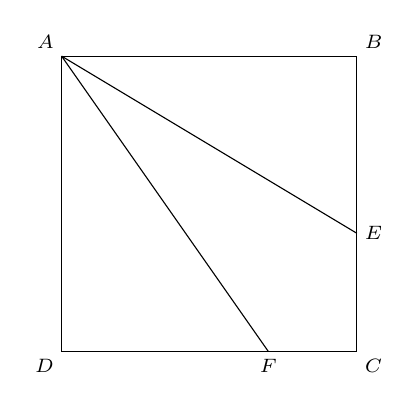
\begin{tikzpicture}[scale=0.75]
        \coordinate (A) at (0,5); \coordinate (B) at (5,5); \coordinate (C) at (5,0); \coordinate (D) at (0,0);
        \draw (A) -- (B) -- (C) -- (D) -- cycle;
        \coordinate (E) at (5,2); \coordinate (F) at (3.5,0);
        \draw (A) -- (E); \draw (A) -- (F);
        \begin{scriptsize}
            \draw (A) node[above left] {$A$}; \draw (B) node[above right] {$B$}; \draw[below right] (C) node {$C$};
            \draw (D) node[below left] {$D$}; \draw[right] (E) node {$E$}; \draw (F) node[below] {$F$};
        \end{scriptsize}
    \end{tikzpicture}
\end{center}

\begin{enumerate}
    \item À quel intervalle appartient $x$ ?
    \item Calculer $AF^2$.
    \item Exprimer $FE^2$ en fonction de $x$.
    \item Montrer que $AE^2 = x^2 - 20x + 200$.
    \item Déterminer la valeur de $x$ pour laquelle le triangle $AFE$ est rectangle en $F$.
\end{enumerate}\[*\]

\exo
On considère un cercle de rayon $\sqrt 7$. On donne les encadrements suivants à $10^{-3}$ près :
\[3{,}141 \leq \pi \leq 3{,}142 \qetq 2{,}645 \leq \sqrt7 \leq 2{,}646.\]
\begin{enumerate}
    \item Donner un encadrement du périmètre $\mtc P$ du cercle à $10^{-1}$ près.
    \item Donner un encadrement de l'aire $\mtc A$ du cercle à $10^{-1}$ près.
\end{enumerate}\[***\]

\end{document} \clearpage
%------ Chapitre 02 - Coordonnées
        \input{02_Fiche02_Coordonnees.tex}\clearpage
%------ Chapitre 03 - Généralités sur les fonctions
        \documentclass[10pt,openright,twoside,french]{book}

\usepackage{marvosym}
\input philippe2013
\input philippe2013_activites

\pagestyle{empty}

\begin{document}

\TitreExo{3}{Généralités sur les \\ fonctions}

\exo Soit $f$ la fonction définie sur l'intervalle $\calig D_f$ dont la courbe représentative $\calig C_f$ est donnée ci-dessous.

\begin{center}
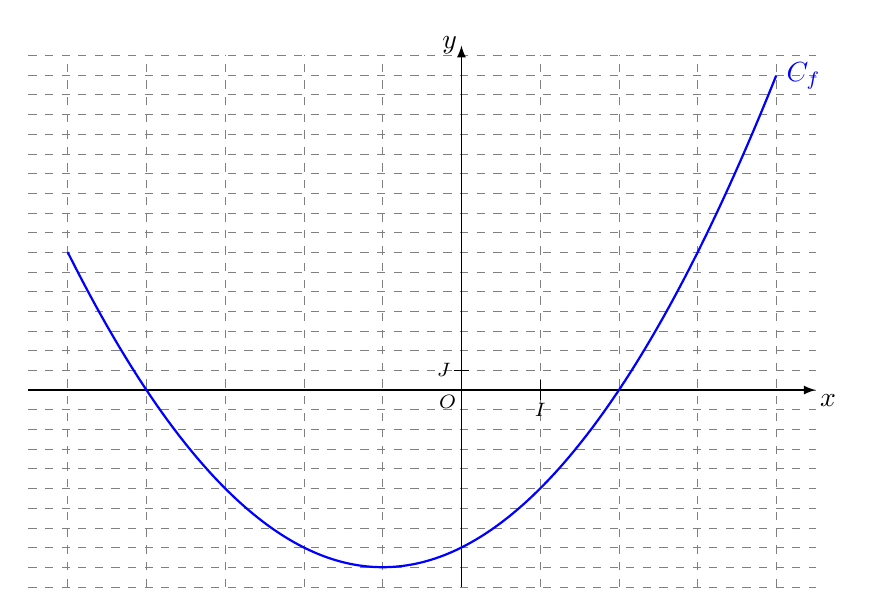
\begin{tikzpicture}[>=latex,yscale=0.25]
    \draw[help lines,dashed] (-5.5,-10) grid (4.5,17);
    \draw[line width=0.5pt,->] (-5.5,0) -- (4.5,0) node[below right=-2pt] {$x$};
    \draw[line width=0.5pt,->] (0,-10) -- (0,17.5) node[left=-2pt] {$y$};
    \draw (1,-0.5) -- (1,0.5); \draw (-0.1,1)--(0.1,1);
    \begin{scriptsize}
    \draw (0,0) node[below left=-1pt] {$O$};
    \draw (1,0) node[below=2pt] {$I$};
    \draw (0,1) node[left=1pt] {$J$};
    \end{scriptsize}
    \draw[blue,thick,domain=-5:4,samples=200]plot(\x,{(\x+1)^2 - 9}) node[right] {$\calig C_f$};
\end{tikzpicture}
\end{center}

\begin{enumerate}
    \item \textbf{Par lecture graphique :}
    \begin{enumerate}
        \item Donner l'intervalle de définition $\calig D_f$.
        \item Donner l'image de $-5$ par la fonction $f$.
        \item Déterminer $f(-2)$.
        \item Dire si le point $A(-3 \pv -5)$ appartient à $\calig C_f$.
        \item Déterminer, s'ils existent, les antécédents des nombres suivants : $16$ ; $0$ ; $-10$.
    \end{enumerate}
    \item \textbf{Par le calcul :} la fonction $f$ est définie pour tout $x \in \R$ par $f(x) = (x + 1)^2 - 9$.
    \begin{enumerate}
        \item Calculer $f(1)$.
        \item Calculer l'image de $\frac 74$ par la fonction $f$.
        \item Résoudre l'équation $f(x) = 0$.
        \item Calculer les antécédents du nombre $-8$.
        \item Déterminer par le calcul si le point $B\left(\frac12 \pv -6\right)$ appartient à la $\calig C_f$.
    \end{enumerate}
\end{enumerate}

\exo On considère la fonction $g$ définie pour tout $x \in \calig D_g$ par $g(x) = \sqrt{3x - 6}$.
\begin{enumerate}
    \item Résoudre l'inéquation $3x - 6 < 0$.
    \item Déterminer $\calig D_g$, ensemble de définition de $g$.
    \item Calculer $g(3)$. Peut-on calculer $g(1)$ ?
    \item Donner les antécédents des nombres $5$ et $-2$.
\end{enumerate}

\exo\medskip

\begin{minipage}{0.45\linewidth}
On donner l'algorithme suivant :
\begin{center}
\small
    \psframebox{
    \parbox{0.8\linewidth}{
        \textbf{Variables}\par
            \quad $x, a, b, c$ : nombres réels\par
        \textbf{Entrée}\par
            \quad Saisir $x$\par
        \textbf{Traitement}\par
            \quad Affecter à $a$ la valeur $x^2$\par
            \quad Affecter à $b$ la valeur $2x$ \par
            \quad Affecter à $c$ la valeur $a-b-3$\par
        \textbf{Sortie}\par
            \quad Afficher $c$
    }}
\end{center}
\end{minipage}
\begin{minipage}{0.53\linewidth}
\begin{enumerate}
    \item Quelle est la fonction $h$ définie par cet algorithme ?
    \item À l'aide de la calculatrice, écrire le tableau de valeurs de cette fonction entre $-2$ et $4$ avec une graduation de $0,5$.
    \item Représenter la fonction $h$ dans un repère orthonormé $\OIJ$ en choisissant \textbf{deux carreaux} comme unité.
\end{enumerate}
\end{minipage}
\end{document} 

\clearpage
\strut
\pieddepage{}{}{}
\entete{}{}{}
\vspace{\stretch{1}}

\[***\]

\begin{center}
\'Ecrit par Philippe \bsc{De Sousa}.\par
Dernière modification le \today.
\end{center}

\end{document} 